% This LaTeX was auto-generated from MATLAB code.
% To make changes, update the MATLAB code and export to LaTeX again.

\documentclass{article}

\usepackage[utf8]{inputenc}
\usepackage[T1]{fontenc}
\usepackage{lmodern}
\usepackage{graphicx}
\usepackage{color}
\usepackage{listings}
\usepackage{hyperref}
\usepackage{amsmath}
\usepackage{amsfonts}
\usepackage{epstopdf}
\usepackage[table]{xcolor}
\usepackage{matlab}

\sloppy
\epstopdfsetup{outdir=./}
\graphicspath{ {./getOlCalendar_images/} }

\begin{document}

\matlabtitle{はじめに}

\begin{par}
\begin{flushleft}
人手不足の昨今、『業務負荷の見える化』を求められてはいませんか。
\end{flushleft}
\end{par}

\begin{par}
\begin{flushleft}
だのに職場が古風で、プロジェクト管理ツールなど導入されてはいない。
\end{flushleft}
\end{par}

\begin{par}
\begin{flushleft}
あるいは導入されたプロジェクト管理ツールがイケてなくて、ぜんぜん定着していない。
\end{flushleft}
\end{par}

\begin{par}
\begin{flushleft}
そんな時、あなたならどうしますか?
\end{flushleft}
\end{par}


\vspace{1em}
\begin{par}
\begin{flushleft}
私「うーん、予定はOutlookで管理してるから、そのデータを負荷の見える化にも使えないものか…」
\end{flushleft}
\end{par}

\begin{par}
\begin{flushleft}
私「…せや!MATLABで解決したらええんや!」
\end{flushleft}
\end{par}

\begin{par}
\begin{flushleft}
私「テキストディープラーニング使えば何か出来るやろ、\href{https://qiita.com/aoimidori/items/796db2e0ce90f64f30d1}{Advent Calendar}にそういうのあったし。」
\end{flushleft}
\end{par}


\vspace{1em}
\begin{par}
\begin{flushleft}
ということで、MATLABで解決していきます。
\end{flushleft}
\end{par}

\begin{par}
\begin{flushleft}
まず本稿では、Outlookから予定表をぶっこ抜くMATLABに持ってくるまでを示します。
\end{flushleft}
\end{par}


\vspace{1em}
\begin{par}
\begin{flushleft}
なお、コードの大半は下記URLを参考に作成しています。
\end{flushleft}
\end{par}

\begin{par}
\begin{flushleft}
そのままだと動かなかったのでメンテしたり加筆したりしました。
\end{flushleft}
\end{par}

\begin{par}
\begin{flushleft}
\href{https://stackoverflow.com/questions/40429116/retrieving-outlook-calendar-items-using-matlab}{https://stackoverflow.com/questions/40429116/retrieving-outlook-calendar-items-using-matlab}
\end{flushleft}
\end{par}


\vspace{1em}
\begin{par}
\begin{flushleft}
またこの記事は井上さんのlivescript2markdownを使って作成しています、便利!
\end{flushleft}
\end{par}

\begin{par}
\begin{flushleft}
\href{https://github.com/minoue-xx/livescript2markdown}{https://github.com/minoue-xx/livescript2markdown}
\end{flushleft}
\end{par}


\vspace{1em}
\begin{matlabcode}
clear all;
close all;
\end{matlabcode}


\matlabheading{1. Outlook APIに接続}

\begin{par}
\begin{flushleft}
下記コマンドを実行することで、MATLABからOutlook APIに接続します。
\end{flushleft}
\end{par}

\begin{matlabcode}
outlook = actxserver('Outlook.Application');
mapi = outlook.GetNamespace('mapi');
\end{matlabcode}

\begin{par}
\begin{flushleft}
次に、GetDefaultFolderkメソッドを叩いてOutlookの所定のフォルダにアクセスします。
\end{flushleft}
\end{par}

\begin{par}
\begin{flushleft}
メソッドの引数とフォルダの対応表は下記URLを参考、予定表フォルダは「9」にあります。
\end{flushleft}
\end{par}

\begin{par}
\begin{flushleft}
\href{https://baccholog.com/archives/128}{Baccho Log [WSH]Outlookの操作}
\end{flushleft}
\end{par}

\begin{matlabcode}
explorer = mapi.GetDefaultFolder(9).GetExplorer;
\end{matlabcode}

\begin{par}
\begin{flushleft}
さらに掘り下げていくことで、個人用や共用の予定表を取得することが出来ます。
\end{flushleft}
\end{par}

\begin{par}
\begin{flushleft}
今回は個人用の予定表を取得してみましょう。
\end{flushleft}
\end{par}

\begin{matlabcode}
NavModule = explorer.NavigationPane.Modules.GetNavigationModule(1); %予定表を取得
NavGroup = NavModule.NavigationGroups.GetDefaultNavigationGroup(1);% 個人用の予定表を取得
%NavGroup = NavModule.NavigationGroups.GetDefaultNavigationGroup(2);% 共用の予定表を取得
\end{matlabcode}


\matlabheading{2.特定の日時でフィルタする}

\begin{par}
\begin{flushleft}
『yyyy/MM/dd HH:mm』または『MM/dd/yyyy HH:mm』のフォーマットで日付を指定します。
\end{flushleft}
\end{par}

\begin{par}
\begin{flushleft}
HH:mmは省略可能ですが(その場合AM8:00ぐらいに指定?)変な結果が出ないよう省略しないのが吉です。
\end{flushleft}
\end{par}

\begin{par}
\begin{flushleft}
またフィルタは予定の開始時間あるいは終了時間で設定できます。開始時間でフィルタする場合は下記。
\end{flushleft}
\end{par}

\begin{matlabcode}
StartDate_MIN = '2020/02/05 00:00';
StartDate_MAX = '2020/02/06 23:00';

%[Start]は開始時間、[End]は終了時間をフィルタ条件として使用
filter = {['[Start] >= ''',StartDate_MIN,''' AND [Start] <= ''', StartDate_MAX, '''']};
\end{matlabcode}


\matlabheading{3.予定を取得、MATLABのテーブルに成型する}

\begin{par}
\begin{flushleft}
取得の対象となるOutlook予定表は下記です。
\end{flushleft}
\end{par}

\begin{par}
\begin{flushleft}
フィルタ条件を2/5\textasciitilde{}2/6に指定したので、「家族と朝ごはん」以降の予定が取れれば成功です。
\end{flushleft}
\end{par}

\begin{par}
\begin{flushleft}
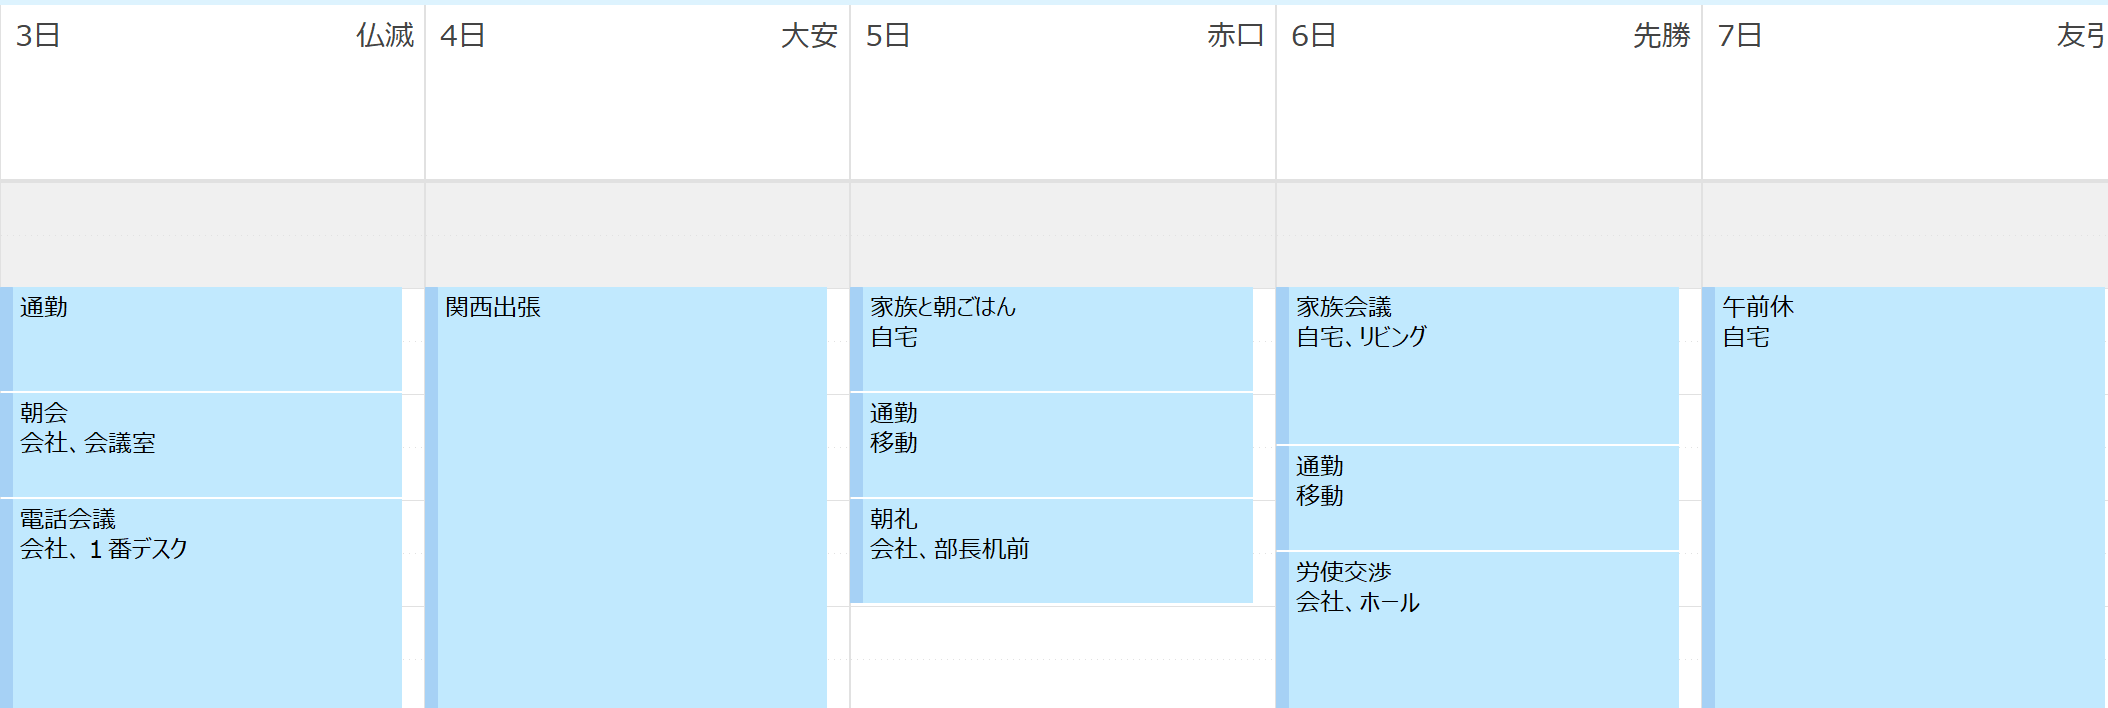
\includegraphics[width=\maxwidth{81.685900652283em}]{image_0}
\end{flushleft}
\end{par}


\vspace{1em}
\begin{par}
\begin{flushleft}
取得およびテーブルの成型は下記。
\end{flushleft}
\end{par}

\begin{par}
\begin{flushleft}
テーブル成型は色々なやり方があるとは思いますが、今回の場合はこれが一番可読性が高いかなと。
\end{flushleft}
\end{par}

\begin{matlabcode}
for i=1:NavGroup.NavigationFolders.Count
    NavFolder = NavGroup.NavigationFolders.Item(i);
    LST = NavFolder.Folder.Items;
    %LST.IncludeRecurrences = -1;
    LST.Sort('[Start]');
    LST_Restrict = LST.Restrict(filter{1});
    Cnt = LST_Restrict.Count;
    sz = [Cnt 3];
    varNames = {'Subject','Start','End'};
    varTypes = {'string','datetime','datetime'};
    Calendar_Table = table('Size',sz,'VariableTypes',varTypes,'VariableNames',varNames);
    for j = 1:Cnt
        Calendar_Table.Subject(j) = LST_Restrict.Item(j).Subject;
        Calendar_Table.Start(j) = LST_Restrict.Item(j).Start;
        Calendar_Table.End(j) = LST_Restrict.Item(j).End;
    end
end

Calendar_Table
\end{matlabcode}
\begin{matlabtableoutput}
{
\begin{tabular} {|c|c|c|c|}\hline
\mlcell{ } & \mlcell{Subject} & \mlcell{Start} & \mlcell{End} \\ \hline
\mlcell{1} & \mlcell{"家族と朝ごはん"} & \mlcell{2020/02/05 08:00:00} & \mlcell{2020/02/05 09:00:00} \\ \hline
\mlcell{2} & \mlcell{"通勤"} & \mlcell{2020/02/05 09:00:00} & \mlcell{2020/02/05 10:00:00} \\ \hline
\mlcell{3} & \mlcell{"朝礼"} & \mlcell{2020/02/05 10:00:00} & \mlcell{2020/02/05 11:00:00} \\ \hline
\mlcell{4} & \mlcell{"家族会議"} & \mlcell{2020/02/06 08:00:00} & \mlcell{2020/02/06 09:30:00} \\ \hline
\mlcell{5} & \mlcell{"通勤"} & \mlcell{2020/02/06 09:30:00} & \mlcell{2020/02/06 10:30:00} \\ \hline
\mlcell{6} & \mlcell{"労使交渉"} & \mlcell{2020/02/06 10:30:00} & \mlcell{2020/02/06 12:00:00} \\ 
\hline
\end{tabular}
}
\end{matlabtableoutput}

\begin{par}
\begin{flushleft}
やったぜ。
\end{flushleft}
\end{par}


\matlabheading{4.予定の長さを計算する}

\begin{par}
\begin{flushleft}
最終ゴールが「業務負荷の見える化」なので、それぞれの予定の長さが知りたいですね。
\end{flushleft}
\end{par}

\begin{par}
\begin{flushleft}
MATLABさんは気が利いているので、下記にて簡単に計算可能です。
\end{flushleft}
\end{par}

\begin{matlabcode}
Calendar_Table.Duration = Calendar_Table.End - Calendar_Table.Start
\end{matlabcode}
\begin{matlabtableoutput}
{
\begin{tabular} {|c|c|c|c|c|}\hline
\mlcell{ } & \mlcell{Subject} & \mlcell{Start} & \mlcell{End} & \mlcell{Duration} \\ \hline
\mlcell{1} & \mlcell{"家族と朝ごはん"} & \mlcell{2020/02/05 08:00:00} & \mlcell{2020/02/05 09:00:00} & \mlcell{01:00:00} \\ \hline
\mlcell{2} & \mlcell{"通勤"} & \mlcell{2020/02/05 09:00:00} & \mlcell{2020/02/05 10:00:00} & \mlcell{01:00:00} \\ \hline
\mlcell{3} & \mlcell{"朝礼"} & \mlcell{2020/02/05 10:00:00} & \mlcell{2020/02/05 11:00:00} & \mlcell{01:00:00} \\ \hline
\mlcell{4} & \mlcell{"家族会議"} & \mlcell{2020/02/06 08:00:00} & \mlcell{2020/02/06 09:30:00} & \mlcell{01:30:00} \\ \hline
\mlcell{5} & \mlcell{"通勤"} & \mlcell{2020/02/06 09:30:00} & \mlcell{2020/02/06 10:30:00} & \mlcell{01:00:00} \\ \hline
\mlcell{6} & \mlcell{"労使交渉"} & \mlcell{2020/02/06 10:30:00} & \mlcell{2020/02/06 12:00:00} & \mlcell{01:30:00} \\ 
\hline
\end{tabular}
}
\end{matlabtableoutput}

\begin{par}
\begin{flushleft}
今回はここまで!
\end{flushleft}
\end{par}


\matlabheading{おわりに}

\begin{par}
\begin{flushleft}
業務効率化ツール、世に出回っているもので十分目的は果たせると思います。が、自分で作ればピンポイントで効果のあるものができてよろしいかと。そして何より楽しいです。
\end{flushleft}
\end{par}

\end{document}
